% Template for Cogsci submission with R Markdown

% Stuff changed from original Markdown PLOS Template
\documentclass[10pt, letterpaper]{article}

\usepackage{cogsci}
\usepackage{pslatex}
\usepackage{float}
\usepackage{caption}

% amsmath package, useful for mathematical formulas
\usepackage{amsmath}

% amssymb package, useful for mathematical symbols
\usepackage{amssymb}

% hyperref package, useful for hyperlinks
\usepackage{hyperref}

% graphicx package, useful for including eps and pdf graphics
% include graphics with the command \includegraphics
\usepackage{graphicx}

% Sweave(-like)
\usepackage{fancyvrb}
\DefineVerbatimEnvironment{Sinput}{Verbatim}{fontshape=sl}
\DefineVerbatimEnvironment{Soutput}{Verbatim}{}
\DefineVerbatimEnvironment{Scode}{Verbatim}{fontshape=sl}
\newenvironment{Schunk}{}{}
\DefineVerbatimEnvironment{Code}{Verbatim}{}
\DefineVerbatimEnvironment{CodeInput}{Verbatim}{fontshape=sl}
\DefineVerbatimEnvironment{CodeOutput}{Verbatim}{}
\newenvironment{CodeChunk}{}{}

% cite package, to clean up citations in the main text. Do not remove.
\usepackage{cite}

\usepackage{color}

% Use doublespacing - comment out for single spacing
%\usepackage{setspace}
%\doublespacing


% % Text layout
% \topmargin 0.0cm
% \oddsidemargin 0.5cm
% \evensidemargin 0.5cm
% \textwidth 16cm
% \textheight 21cm

\title{Drawings as a window into developmental changes in object
representations}


\author{{\large \bf Bria Long} \\ \texttt{bria@stanford.edu} \\ Department of Psychology \\ Stanford University \And {\large \bf Judith E. Fan} \\ \texttt{jefan@stanford.edu} \\ Department of Psychology \\ Stanford University \And {\large \bf Michael C. Frank } \\ \texttt{mcfrank@stanford.edu} \\ Department of Psychology \\ Stanford University}

\begin{document}

\maketitle

\begin{abstract}
How do children's representations of object categories change as they
grow older? As they learn about the world around them, they also express
what they know in the drawings they make. Here, we examine drawings as a
window into how children represent familiar object categories, and how
this changes across childhood. We asked children (age 3-10 years) to
draw familiar object categories on an iPad. First, we analyzed their
semantic content, finding large and consistent gains in how well
children could produce drawings that are recognizable to adults. Second,
we quantified their perceptual similarity to adult drawings using a
pre-trained deep convolutional neural network, allowing us to visualize
the representational layout of object categories across age groups using
a common feature basis. We found that the organization of object
categories in older children's drawings were more similar to that of
adults than younger children's drawings. This correspondence was strong
in the final layers of the neural network, showing that older children's
drawings tend to capture the perceptual features critical for adult
recognition. We hypothesize that this improvement reflects increasing
convergence between children's representations of object categories and
that of adults; future work will examine how these age-related changes
relate to children's developing perceptual and motor capacities.
Broadly, these findings point to drawing as a rich source of insight
into how children represent object concepts.

\textbf{Keywords:}
object representations; drawings; child development
\end{abstract}

\newcommand{\wrapmf}[1]{#1} 





\section{Introduction}\label{introduction}

As humans, we have many powerful tools to externalize what we know,
including language and gesture. One tool that has been transformative
for human cognition and culture is graphical representation, which
allows people to encode their thoughts in a visible, durable format.
Drawing is an important case study in graphical representation, being a
technique that dates back 60,000 years (Hoffmann et al., 2018), well
before the emergence of symbolic writing systems, and is practiced in
many cultures.

In modern times, drawings are produced prolifically by children from an
early age, providing a rich source of potential insight into their
emerging understanding of the visual world. For example, as children
learn the diagnostic properties of objects they encounter, they might
express this knowledge in the drawings they make. How can we leverage
this natural behavior to understand how they learn abstractions over
their perceptual experience, such as object categories?

On the one hand, children quickly form sophisticated perceptual
representations of familiar objects, leveraging shape information in
conjunction with linguistic cues (Smith, Jones, Landau, Gershkoff-Stowe,
\& Samuelson, 2002). Typically, such learning is measured using discrete
choices between stimuli that vary along dimensions chosen by an
experimenter. By contrast, drawing tasks both permit children to include
any information they consider relevant and can provide rich,
high-dimensional information about the content and structure of
children's perceptual representations. For example, when presented with
a target object to draw in which a prominent feature is occluded (e.g.,
the handle of a mug is turned away), children as young as 5 years of age
frequently include the occluded object part in their drawing anyway,
displaying the robustness of their internal representation to variation
in viewpoint (Davis, 1983).

On the other hand, important developmental changes in perceptual
processing continue throughout childhood (for reviews, see Juttner,
Wakui, Petters, \& Davidoff, 2016; Nishimura, Scherf, \& Behrmann,
2009). For example, young children tend to categorize novel objects on
the basis of part-specific information, whereas older children
additionally recruit information about relationships between object
parts (Mash, 2006). Such differences are resonant with evidence from
children's drawings: there appear to be dramatic changes in how children
encode semantically relevant information in their drawings across age.
Younger children (4-5 years) tend to include fewer cues in their
drawings to differentiate between target concepts (e.g., ``adult'' vs.
``child'') than older children, who enrich their drawings with more
diagnostic part (Sitton \& Light, 1992) or relational (Light \& Simmons,
1983) information.

\begin{CodeChunk}
\begin{figure*}[h]

{\centering 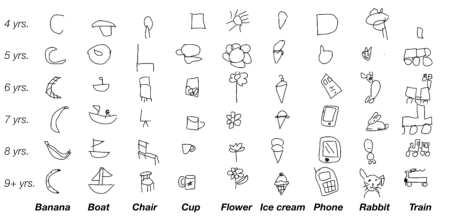
\includegraphics[width=1\linewidth]{figs/exampleDrawings-1} 

}

\caption[Example drawings made by children ages 4-10 of several object categories]{Example drawings made by children ages 4-10 of several object categories.}\label{fig:exampleDrawings}
\end{figure*}
\end{CodeChunk}

But while figurative drawings have long provided inspiration for
scientists investigating the representation of object concepts in early
life (Minsky \& Papert, 1972), a major barrier has been the lack of
principled quantitative measures of high-level perceptual information in
drawings. As such, previous studies employing drawing tasks have
typically relied on qualitative assessments (Kosslyn, Heldmeyer, \&
Locklear, 1977) or ad hoc quantitative criteria (Goodenough, 1963).
Recent work in computational vision has validated the use of pre-trained
deep convolutional neural network (DCNN) models to quantitatively
measure high-level perceptual information in adult drawings (Fan,
Yamins, \& Turk-Browne, 2015). Higher layers of these models both
capture adult perceptual judgments of object shape similarity (Kubilius,
Bracci, \& Op de Beeck, 2016) and predict neural population responses in
categories throughout object-selective cortex (Yamins et al., 2014).
Thus, features learned by these models provide a principled choice of
basis for extracting perceptual features useful for inferring object
identity from children's drawings.

Here we examine children's drawings as a window into how they represent
familiar visual object categories, and how this representation and its
translation into graphical form changes across childhood. To do so, we
asked children (ages 3-10 years) to draw a variety of object categories
on a digital tablet. Afterwards, adults attempted to recognize these
drawings in a forced-choice recognition task. In Part 1, we examine how
this semantic information in children's drawings changes with age after
factoring out low-level covariates related to motor production, such as
how long they spend drawing and how many strokes they use. In Part 2, we
compare the high-level perceptual features of drawings made by children
and adults by relating their representations in a pre-trained DCNN
model, allowing us to visualize the representational layout of object
categories across age groups using a common feature basis.

\section{Part 1: Semantic information in children's
drawings}\label{part-1-semantic-information-in-childrens-drawings}

\subsection{Methods}\label{methods}

\subsubsection{Participants}\label{participants}

For the drawing task, children (N = 41, M = 6.9 years, range 4-10 years)
were recruited at the San Jose Children's Discovery Museum. Either the
child or their parents verbally reported the child's age. For the
recognizability experiment, 14 naive adults with US IP addresses were
recruited from Amazon Mechanical Turk and provided labels for all
drawings.

\subsubsection{Stimuli}\label{stimuli}

Stimuli were words referring to 16 common object categories: banana,
boat, car, carrot, cat, chair, couch, cup, flower, foot, frog, ice
cream, phone, rabbit, shoe, train. These categories were chosen such
that they were: (1) likely to be familiar to children, (2) spanned the
animate/inanimate distinction, and (3) intuitively spanned a wide range
of difficulty (for example, flowers seem easier to draw than couches).
We also chose categories that are in the Google QuickDraw database,
which contains drawings made by adults in under 20 seconds, so that we
could eventually compare children's drawings with ones made by adults.

\subsubsection{Drawing Task Procedure}\label{drawing-task-procedure}

We implemented a web-based drawing game in HTML/Javascript using the
paper.js library and collected drawings using a touchscreen tablet on
the floor of the museum. At the beginning of each session, to
familiarize children with the task and touch interface, they were
prompted to draw a circle and a triangle. After completing these two
practice trials, they were cued to draw a randomly selected object. On
each trial, a text cue would appear (i.e., ``Can you draw a
{[}flower{]}?'') that the experimenter would read out, (``What about a
{[}flower{]}? Can you draw a {[}flower{]}?). Then, a drawing canvas
appeared (600 x 600 pixels) and children had 30 seconds to make a
drawing before moving onto the next trial; pilot testing suggested that
30 seconds was enough for many children to complete their drawings.
After each trial, the experimenter asked the child whether they wanted
to keep drawing or whether they were all done. In all, we collected 286
drawings across the 16 categories. We binned drawings into two rough age
categories for item analyses, with 115 drawings made by younger children
(4-6 years of age) and 171 drawings made by older children (7-10 years
of age).

\subsubsection{Recognizability Task
Procedure}\label{recognizability-task-procedure}

After collecting children's drawings, we presented them to naive adults
to measure their recognizability. On each trial, participants saw a
drawing, and were asked ``What does this look like?'', and responded by
typing their response into a text box. Only labels from a restricted set
of 21 options were accepted, comprising the 16 drawn categories, 4 foil
categories (bean, arm, person, rock), and ``cannot tell at all.''
Drawings were presented in a random order, and participants were not
informed that these drawings were produced by children.

\subsubsection{Model Fitting}\label{model-fitting}

Our goal was to measure how children's ability to convey semantically
relevant information in their drawings changes with age. We anticipated
that their drawings may also vary along other dimensions more directly
related to the motor production demands of the task, such as the amount
of time spent drawing, the number of strokes used, and amount of ink
(i.e., mean pixel intensity of sketch).

In order to assess whether children's ability to produce recognizable
drawings increased with age, independent of these low-level covariates,
we fit a generalized linear mixed-effects model, with scaled age
(specified in years), drawing duration, amount of ink used, and number
of strokes as fixed effects, and with random intercepts for each
individual child and object category. The dependent variable was whether
adults recognized a given drawing.

\begin{table}[H]
\centering
\begin{tabular}{rrrrr}
  \hline
 & Estimate & Std. Error & z value & Pr($>$$|$z$|$) \\
  \hline
(Intercept) & 0.861 & 0.321 & 2.680 & 0.007 \\
  Age & 0.956 & 0.174 & 5.497 & 0.000 \\
  Drawing time & 0.338 & 0.109 & 3.105 & 0.002 \\
  Amount of ink & 0.014 & 0.080 & 0.179 & 0.858 \\
  Num. strokes & -0.289 & 0.098 & -2.959 & 0.003 \\
   \hline
\end{tabular}
\caption{Model coefficients of a GLMM predicting the recognizability of each drawing.}
\end{table}

\begin{CodeChunk}
\begin{figure}[H]

{\centering 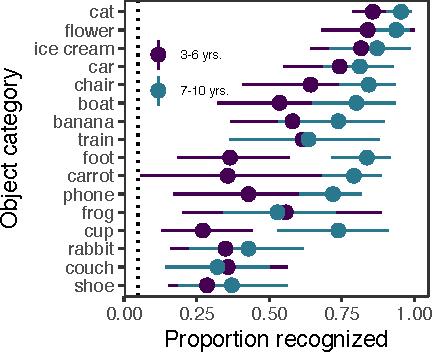
\includegraphics{figs/recognizabilityByItem-1} 

}

\caption[Proportion of drawings recognized in each object category]{Proportion of drawings recognized in each object category. The dashed line represents chance performance. Error bars represent non-parametric 95 \% confidence intervals. }\label{fig:recognizabilityByItem}
\end{figure}
\end{CodeChunk}

\subsection{Results}\label{results}

We found that drawing recognizability generally increased with age (see
Figure \ref{fig:covDescriptives}), although there was substantial
variability across categories in how well children could produce
recognizable drawings. For example, children of all ages produced
drawings of cats that were readily recognizable as ``cats,'' but few
children of any age produced drawings that were recognizable as
``shoes'' (see Figure \ref{fig:recognizabilityByItem}).

Was this difference due to greater semantic information in older
children's drawings, or to the possibility that older children may have
put more time and effort into their drawings? Our mixed-effects model
revealed that recognizability of drawings reliably increased with age
when controlling for these low-level covariates --- the amount of time
spent drawing, the number of strokes, and total ink used (\(\beta\) =
0.96, SE = 0.17, Z = 5.5), and accounting for variation across object
categories and individual children. All model coefficients can be seen
in Table 1. Adding interaction terms between age and these low-level
covariates did little to decrease the effect of age on recognizability
(\(\beta\) = 0.94, SE = 0.18, Z = 5.4).

Taken together, these results show large and consistent gains in how
well children can produce recognizable drawings across this age range,
although younger children still produced drawings that could be
recognized well above chance by adult viewers.

\section{Part 2: Perceptual information in children's
drawings}\label{part-2-perceptual-information-in-childrens-drawings}

In the previous section, we found that children's drawings generally
contained sufficient semantic information to support recognition by
adult viewers, although older children's drawings were consistently more
recognizable. What is the nature of the developmental changes that
underlie older children's enhanced ability to produce recognizable
drawings (at least to adult viewers)? And how might children's drawings
provide a window into their perceptual representations of these objects?

\begin{CodeChunk}
\begin{figure*}[h]

{\centering 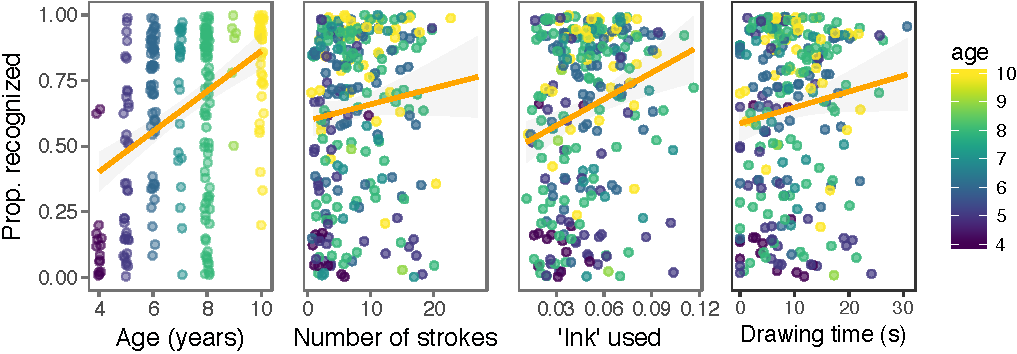
\includegraphics{figs/covDescriptives-1} 

}

\caption[The proportion of adults who recognized each drawing is plotted as a function of child's age, the number of strokes, amount of ink used, and the time spent creating each drawing]{The proportion of adults who recognized each drawing is plotted as a function of child's age, the number of strokes, amount of ink used, and the time spent creating each drawing. Each dot represents an individual drawing; dots in the right three plots are colored by the age of the drawer.}\label{fig:covDescriptives}
\end{figure*}
\end{CodeChunk}

We hypothesized that this improvement reflects an increasing convergence
in the perceptual content in children and adult's drawings, derived from
their internal object representations. A pre-requisite for this
hypothesis is that older children's drawings are more perceptually
similar to adults' drawings than younger children's drawings. We thus
extracted the high-level perceptual features of drawings made by
children and adults using a pre-trained deep convolutional neural
network (Simonyan \& Zisserman, 2014). These features form a common
basis for representing complex shape similarity -- including the
presence of diagnostic object parts (e.g., legs, handles) -- and a basis
from which object identity can be easily derived (Kubilius et al.,
2016). We then use these high-level features to evaluate how similar the
representational layout of object categories is between children's and
adults' drawings. Insofar as the similarity of the representational
layout is higher for older children than younger children, this could
explain why adults are more accurate in recognizing their drawings. As a
sanity check, we also explored how similar children and adult's drawings
are in each layer of the model. Earlier layers reflect local image
properties (e.g., edge orientations) which are then successively
transformed and combined to yield the more abstract mid-level features
(e.g., curvature) and higher-level features represented in later layers.
Thus, these layer-wise analyses can reveal how similar children and
adult's drawings are in terms of more basic statistics---e.g., if both
childrens' and adult's drawings of phones are ``boxier'' than their
drawings of apples.

\subsection{Methods}\label{methods-1}

\subsubsection{Participants}\label{participants-1}

Participants included those who participated in the first round of data
collection, as well as an additional 25 children recruited in the same
way as in Part 1.

\subsubsection{Drawing dataset}\label{drawing-dataset}

In our second round of data collection, our goal was to expand the
number of categories included in our model-based feature analyses, so we
included an additional 22 categories. Across both rounds of data
collection, we recorded 462 drawings from 66 children across a broad age
range. However, due to the limited amount of data in each category for
each age, in subsequent analyses we divide drawing data into two coarse
age categories: younger children (aged 3-6 years) and older children
(aged 7-10 years). We thus restricted the following analyses to the 27
categories where we had at least 3 drawings in both younger and older
age groups, yielding 191 drawings by younger children and 205 drawings
by older children. Including a minimum number of drawings per class and
age category ensured robust estimates of category-level feature
information in drawings.

To complement the children's drawing dataset, we obtained a random
sample of 100 adult drawings from each of the categories above from the
Google Quickdraw dataset (\url{https://quickdraw.withgoogle.com/data}).
Prior to analysis, we cropped all sketch images to contain only the
sketch, applied uniform padding (10px), and rescaled them to the same
size (3x224x224).

\subsubsection{Deep convolutional neural network
model}\label{deep-convolutional-neural-network-model}

We used a standard, pre-trained implementation of the VGG-19
architecture (Simonyan \& Zisserman, 2014) to extract features from
sketches at layers across several depths in the network. Specifically,
we analyzed feature activations in the first five pooling layers, as
well as the first two fully-connected layers. Each image elicits a
pattern of feature activations at every layer in the model. Here, we sum
across the spatial position of the image filters to reduce
dimensionality; thus, each pattern is equivalent to a vector in a
feature space with the same number of dimensions as convolutional
filters in that layer.

\begin{CodeChunk}
\begin{figure*}[h]

{\centering 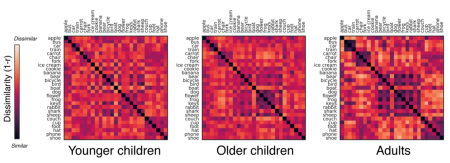
\includegraphics[width=1\linewidth]{figs/RSAAllCat-1} 

}

\caption[Representational dissimilarity matrices (RDMs) in the highest layer of VGG-19 (FC7) for drawings made by younger children (3-6 years), older children (7-10 years), and adults]{Representational dissimilarity matrices (RDMs) in the highest layer of VGG-19 (FC7) for drawings made by younger children (3-6 years), older children (7-10 years), and adults.}\label{fig:RSAAllCat}
\end{figure*}
\end{CodeChunk}

\subsubsection{Representational Similarity
Analyses}\label{representational-similarity-analyses}

Separately for the younger children, older children, and adult drawing
datasets, we averaged the feature vectors within each object category in
both pixel space and for a given layer of VGG-19 and then computed a
layer-specific matrix of the Pearson correlation distances between these
average vectors across categories (Kriegeskorte, Mur, \& Bandettini,
2008). Formally, this entailed computing:
\[RDM(R)_{ij} = 1- \frac{cov(\vec{r}_{i}, \vec{r}_{j})}{\sqrt{var(\vec{r}_{i}) \cdot var(\vec{r}_{j})}},\]
where \(\vec{r}_{i}\) and \(\vec{r}_{j}\) are the mean feature vectors
for the \(i\)th and \(j\)th object categories, respectively, where R
represents the correlation between two categories (e.g., rabbits and
shoes).

Each of these 27x27 representational dissimilarity matrices (RDM)
provides a compact description of the layout of objects in the
high-dimensional feature space inherent to each layer of the model.
Following Kriegeskorte et al. (2008), we measured the similarity between
object representations in different layers by computing the Spearman
rank correlations between the RDMs for those corresponding layers.
Estimates of standard error for the Spearman correlation between RDMs
were generated by jackknife resampling of the 27 object categories. To
estimate the noise ceiling, we repeated this same procedure with an
equivalently sized, random sample of adult drawings.

\begin{CodeChunk}
\begin{figure}[H]

{\centering 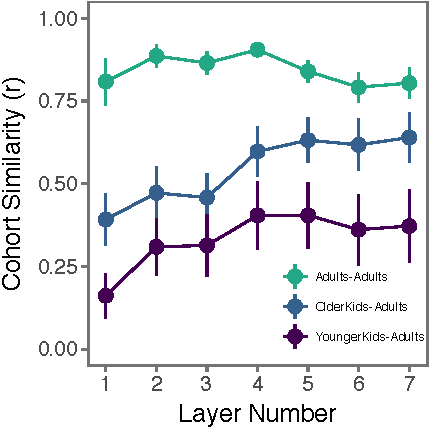
\includegraphics{figs/layerWise-1} 

}

\caption[Spearman's correlation between representational dissimilarity matrices (RDMs) of drawings produced by adults vs]{Spearman's correlation between representational dissimilarity matrices (RDMs) of drawings produced by adults vs. other adults, adults vs. older children, and between adults vs. younger children at each layer of VGG-19. }\label{fig:layerWise}
\end{figure}
\end{CodeChunk}

\subsection{Results}\label{results-1}

To compare the representational layout of object categories across age
groups, we examined the similarity between RDMs for each age group
(i.e., younger children, older children, and adults) in the final layer
of VGG-19, shown in Figure \ref{fig:RSAAllCat}. Here, each cell
represents the correlation distance between two categories in this layer
of the network; lighter colors indicate pairs of categories that are
further apart in feature space; darker colors indicate pairs of
categories that are closer. For visualization purposes, categories are
ordered according to the clusters that appear in the data. Inspecting
the similarity structure for adults, drawings of living things (rabbits,
frogs, flowers, etc.) elicited the most similar representations, evident
in a cluster in the middle of the RDM. While there are some intuitive
category clusters (bus--car--train), other clusters seem less intuitive
at first blush (carrot--chair--ice cream--fork)---yet note that these
categories tend to have a similar aspect ratio. Importantly, this
perceptual similarity structure was echoed in children's drawings of
these same object categories.

We then examined these correlations between RDMs at each layer of the
network, which are plotted in Figure \ref{fig:layerWise} relative to the
comparison between two samples of adult drawings, representing the noise
ceiling. We found that older children's and adults' RDMs were more
similar than younger children's and adult's RDMs across all layers, and
that similarity plateaued in mid-to-high-level convolutional layers (see
Figure \ref{fig:layerWise}). These results suggest that the particular
choice of model layer does not affect the relative similarity between
older children's and adults' RDMs vs.~younger children's and adults'
RDMs. Nonetheless, adults' and children's drawings were dissimilar in
pixel space for both age groups (adults vs.~older children, r = .07;
vs.~younger children, r = .07). Children's and adults' drawings appear
to share many of the perceptual features useful for object recognition.

\section{General Discussion}\label{general-discussion}

What do children's drawings reveal about their object representations?
We approached this question by analyzing the semantic and perceptual
content of children's drawings across childhood. We found that the
capacity to quickly produce drawings that communicate category
information improves with age, even when factoring out low-level motor
covariates. In addition, we found that drawings from older vs.~younger
children were more similar to adult drawings in a deep convolutional
neural network trained to recognize objects, suggesting that older
children's drawings also contain more of the perceptual features
relevant for recognition. Children and adults may be accessing similar
category representations when asked to ``draw a chair'' and
communicating this representation through their drawings.

A natural question is how any age-related differences in drawings are
related to children's ability to control and plan their hand movements.
While drawing recognizability increased with age when accounting for the
low-level motor covariates, these measures likely only partially
estimate children's motor abilities. We plan to measure both children's
and adult's ability to perform orthogonal fine motor tasks (e.g.,
tracing a complex shape) to understand how motor developments influence
the drawings that children produce.

At the same time, children are also continuously learning about new
object categories and their properties. How might this learning affect
children's internal representations (and drawings) of different object
categories? One possibility is that the bulk of the development change
revolves around building more detailed representations: children may be
learning the suite of visual features and object parts that are
diagnostic of various object categories. On this account, learning what
tigers tend to look like does not change children's perceptual
representations of cheetahs---or how they draw them. A second
possibility is that learning about new categories actually changes the
similarity structure of children's visual object concepts (Goldstone,
Lippa, \& Shiffrin, 2001). Finally, as children learn about the
hierarchical structure of object categories (i.e., living
thing--animal--mammal--dog) and their typical properties (e.g., most
mammals have four legs) this might differentially change which visual
features take precedence in their internal representations. Future work
that links children's categorization abilities with their drawing
behaviors will help explore these possibilities.

This work integrates novel methods to investigate children's internal
representations of object categories and how they are linked to their
developing perceptual, cognitive, and motor abilities. We propose that a
full understanding of how we come to produce visual abstractions will
help uncover the factors that shape adult object representations.

\clearpage

\section{Acknowledgements}\label{acknowledgements}

We thank Jacqueline Quirke and Renata Chai for help with piloting and
data collection. We thank members of Stanford Language and Cognition
lab. This work was funded by an NSF SPRF-FR Grant \#1714726 to BLL and a
Jacobs Foundation Fellowship to MCF. We also gratefully acknowledge
those who made the Google QuickDraw database available.

\section{References}\label{references}

\setlength{\parindent}{-0.1in} \setlength{\leftskip}{0.125in} \noindent

\hypertarget{refs}{}
\hypertarget{ref-davis1983contextual}{}
Davis, A. M. (1983). Contextual sensitivity in young children's
drawings. \emph{Journal of Experimental Child Psychology}, \emph{35}(3),
478--486.

\hypertarget{ref-fan2015common}{}
Fan, J. E., Yamins, D., \& Turk-Browne, N. B. (2015). Common object
representations for visual recognition and production. \emph{Proceedings
of the 37th Proceedings of Annual Conference of the Cognitive Science
Society.}

\hypertarget{ref-goldstone2001altering}{}
Goldstone, R. L., Lippa, Y., \& Shiffrin, R. M. (2001). Altering object
representations through category learning. \emph{Cognition},
\emph{78}(1), 27--43.

\hypertarget{ref-goodenough1963goodenough}{}
Goodenough, F. L. (1963). \emph{Goodenough-harris drawing test}.
Harcourt Brace Jovanovich New York.

\hypertarget{ref-hoffmann2018u}{}
Hoffmann, D. L., Standish, C. D., García-Diez, M., Pettitt, P. B.,
Milton, J., Zilhão, J., \ldots{} others. (2018). U-th dating of
carbonate crusts reveals neandertal origin of iberian cave art.
\emph{Science}, \emph{359}(6378), 912--915.

\hypertarget{ref-juttner2016developmental}{}
Juttner, M., Wakui, E., Petters, D., \& Davidoff, J. (2016).
Developmental commonalities between object and face recognition in
adolescence. \emph{Frontiers in Psychology}, \emph{7}.

\hypertarget{ref-kosslyn1977children}{}
Kosslyn, S. M., Heldmeyer, K. H., \& Locklear, E. P. (1977). Children's
drawings as data about internal representations. \emph{Journal of
Experimental Child Psychology}, \emph{23}(2), 191--211.

\hypertarget{ref-kriegeskorte2008RSA}{}
Kriegeskorte, N., Mur, M., \& Bandettini, P. (2008). Representational
similarity analysis--connecting the branches of systems neuroscience.
\emph{Frontiers in Systems Neuroscience}, \emph{2}.

\hypertarget{ref-kubilius2016deep}{}
Kubilius, J., Bracci, S., \& Op de Beeck, H. P. (2016). Deep neural
networks as a computational model for human shape sensitivity.
\emph{PLoS Computational Biology}, \emph{12}(4), e1004896.

\hypertarget{ref-light1983effects}{}
Light, P., \& Simmons, B. (1983). The effects of a communication task
upon the representation of depth relationships in young children's
drawings. \emph{Journal of Experimental Child Psychology}, \emph{35}(1),
81--92.

\hypertarget{ref-mash2006}{}
Mash, C. (2006). Multidimensional shape similarity in the development of
visual object classification. \emph{Journal of Experimental Child
Psychology}, \emph{95}(2), 128--152.

\hypertarget{ref-minsky1972artificial}{}
Minsky, M., \& Papert, S. A. (1972). Artificial intelligence progress
report.

\hypertarget{ref-nishimura2009}{}
Nishimura, M., Scherf, S., \& Behrmann, M. (2009). Development of object
recognition in humans. \emph{F1000 Biology Reports}, \emph{1}.

\hypertarget{ref-simonyan2014very}{}
Simonyan, K., \& Zisserman, A. (2014). Very deep convolutional networks
for large-scale image recognition. \emph{ArXiv Preprint
ArXiv:1409.1556}.

\hypertarget{ref-sitton1992drawing}{}
Sitton, R., \& Light, P. (1992). Drawing to differentiate: Flexibility
in young children's human figure drawings. \emph{British Journal of
Developmental Psychology}, \emph{10}(1), 25--33.

\hypertarget{ref-smith2002object}{}
Smith, L. B., Jones, S. S., Landau, B., Gershkoff-Stowe, L., \&
Samuelson, L. (2002). Object name learning provides on-the-job training
for attention. \emph{Psychological Science}, \emph{13}(1), 13--19.

\hypertarget{ref-yamins2014performance}{}
Yamins, D., Hong, H., Cadieu, C. F., Solomon, E. A., Seibert, D., \&
DiCarlo, J. J. (2014). Performance-optimized hierarchical models predict
neural responses in higher visual cortex. \emph{Proceedings of the
National Academy of Sciences}, \emph{111}(23), 8619--8624.

\vspace{2em}
\centering{
\fbox{\parbox[b][][c]{7.3cm}{\centering All data and code for these analyses are available at\ \url{https://github.com/brialorelle/kiddraw}}}}
\vspace{1em}

\end{document}
